This layer involves the various sensors and indicators that interact between the Turing Board and the user directly. This includes a load cell or force-sensing resistor for a weight sensor, a piezoelectric speaker, a printed ArUco symbol, a PWM-capable LED strip, a Tiva C Series Microcontroller, and various electrical components. The weight sensor, speaker, and LEDs communicate directly with the Tiva C Series, while the ArUco symbol is recognized by an Intel RealSense camera which sends the data to the Jetson TX2 via the CV Layer. The Tiva C Series is programmed using C and Assembly via Code Composer Studio 10, while the libraries used for the CV layer mainly use C++ and a generic IDE. This is capable of running on both Windows, MacOS, and Linux.

\subsection{Layer Hardware}
This layer uses a generic piezoelectric speaker (buzzer), a load cell or force-sensing resistor (weight sensor), a printed ArUco symbol generated online (follow anklet), a strip of PWM-capable LEDs approximately 10ft in length, a Tiva C Series, and various electrical components (MOSFETs, resistors, ADC, etc.).

\subsection{Layer Operating System}
N/A.

\subsection{Layer Software Dependencies}
This layer depends on code done in Code Composer Studio (v10.2) to program the Tiva C Series and drive the various HMI subsystems. We also used the site https://chev.me/arucogen/ to generate our ArUco symbol.

\subsection{Weight Sensor}
The weight sensor will be implemented as a safety feature primarily, with future uses in load carrying. When a user is riding on the board, it will detect if they fall off to initiate an emergency stop. When a user attempts to get on the board while in autonomous mode it will trigger an alert noise to notify the user it is not safe to ride.

\begin{figure}[h!]
	\centering
 	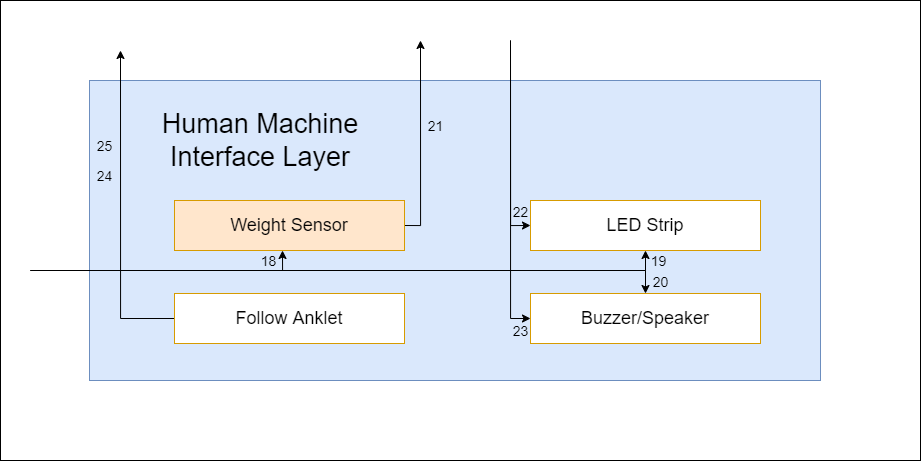
\includegraphics[width=0.60\textwidth]{images/Kendall/Weight Sensor.png}
 \caption{Weight Sensor Subsystem in HMI Layer}
\end{figure}

\subsubsection{Subsystem Hardware}
The weight sensor will implement either a generic load cell or force-sensing resistor in or order to determine the weight/pressure being generated by an item/person placed on top. This will detect and send any weight data to a Tiva C Series to parse and decode.

\subsubsection{Subsystem Operating System}
N/A.

\subsubsection{Subsystem Software Dependencies}
The weight sensor requires the Tiva C Series to read and parse any data. This, in turn, requires Code Composer Studio 10 to create code to parse/read the data and program the Tiva accordingly.

\subsubsection{Subsystem Programming Languages}
Code Composer Studio 10 has code written in C and Assembly.

\subsubsection{Subsystem Data Structures}
The data read in by the sensor is formed into 24-bit "packets" sent along a datastream to the Tiva running at 100kHz. This is done by transmitting one bit per clock using an ADC. This data, which correspond with an external linear force, is then read and parsed by the Tiva and any relevant data is passed to the other subsystems (LEDs and Buzzer/Speaker) to alert of a weight change.

\subsubsection{Subsystem Data Processing}
N/A.

\subsection{Buzzer/Speaker}
The buzzer/speaker will be used to alert the user if they attempt to step on the board when it is in an autonomous mode. When the weight sensor detects a person attempting to stand on the board when in autonomous mode, the buzzer will begin to sound an alert to notify the user it is unsafe to stand on it.

\begin{figure}[h!]
	\centering
 	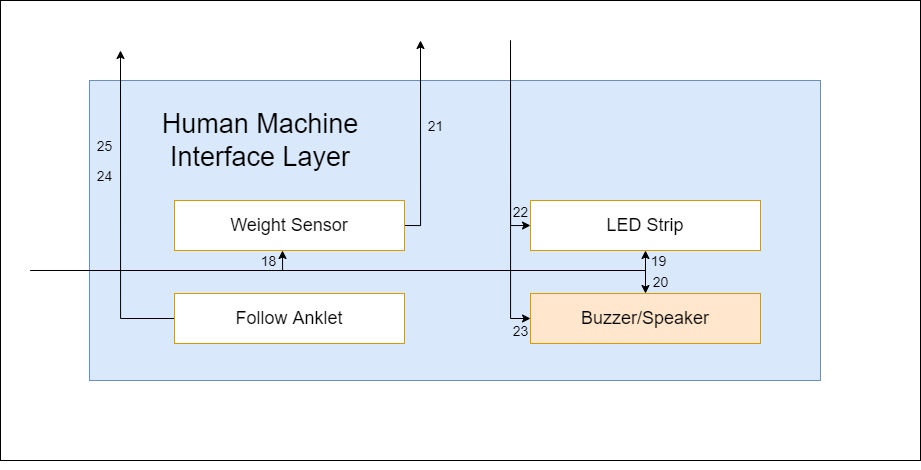
\includegraphics[width=0.60\textwidth]{images/Kendall/Buzzer.png}
 \caption{Buzzer/Speaker Subsystem in HMI Layer}
\end{figure}

\subsubsection{Subsystem Hardware}
This subsystem uses a generic piezoelectric speaker powered and run by a Tiva C Series to emit a sound as an alert on various conditions.

\subsubsection{Subsystem Operating System}
N/A.

\subsubsection{Subsystem Software Dependencies}
Code Composer Studio 10 is used to send signals to the piezoelectric speaker in order to emit a sound of a pre-determined frequency and length.

\subsubsection{Subsystem Programming Languages}
Code Composer Studio 10 has code written in C and Assembly.

\subsubsection{Subsystem Data Structures}
A signal is sent from the Tiva to the speaker using a 32-bit value to determine the frequency at which to emit the sound. The Tiva also uses a 32-bit variable to determine how long to emit the signal for before sending a stop command.

\subsubsection{Subsystem Data Processing}
N/A.

\subsection{LED Strip}
The LED strip will be used to indicate to the user what mode the Turing Board is currently in. These modes will be differentiated by implementing a different color for each mode. 

\begin{figure}[h!]
	\centering
 	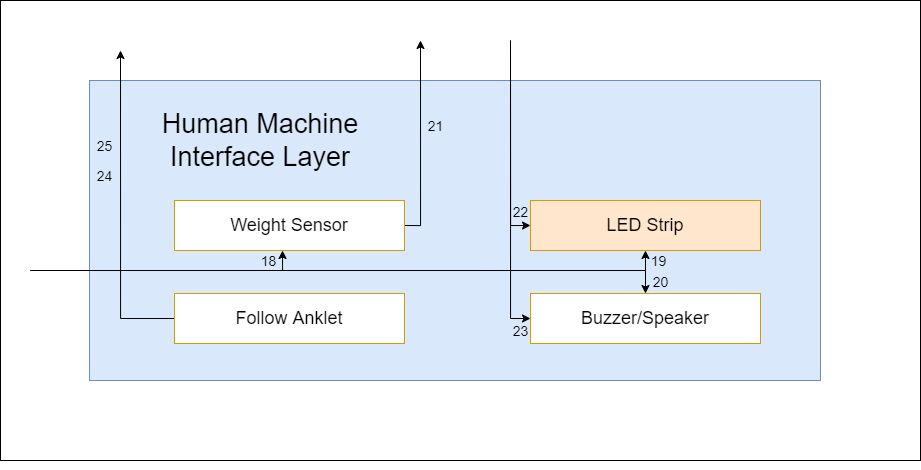
\includegraphics[width=0.60\textwidth]{images/Kendall/LED Strip.png}
 \caption{LED Strip Subsystem in HMI Layer}
\end{figure}

\subsubsection{Subsystem Hardware}
These LEDs are specifically PWM-capable and rated at up to 12V. It also implements a Tiva C Series to control the LEDs.

\subsubsection{Subsystem Operating System}
N/A.

\subsubsection{Subsystem Software Dependencies}
The LEDs are powered and controlled by the Tiva using Code Composer Studio.

\subsubsection{Subsystem Programming Languages}
Code Composer Studio 10 has code written in C and Assembly.

\subsubsection{Subsystem Data Structures}
The LEDs are each fed a 256-bit value corresponding to the Red, Blue, and Green data lines from the Tiva. This, in turn, activates the respective LED color to create various combinations based on each R/G/B input values.

\subsubsection{Subsystem Data Processing}
N/A.

\subsection{Follow Anklet}
The Anklet will be a worn feature used for the CV to track and follow the rider in follow-along mode.

\begin{figure}[h!]
	\centering
 	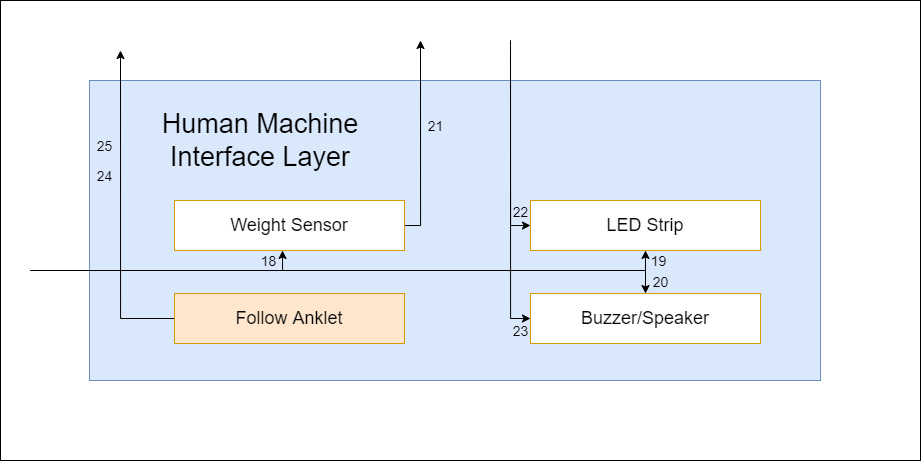
\includegraphics[width=0.60\textwidth]{images/Kendall/Anklet.png}
 \caption{Follow Anklet Subsystem in HMI Layer}
\end{figure}

\subsubsection{Subsystem Hardware}
This subsystem simply uses an ArUco symbol printed out on a strip of paper long enough to wrap around one's ankle.

\subsubsection{Subsystem Operating System}
N/A.

\subsubsection{Subsystem Software Dependencies}
This depends on the ArUco library based on the OpenCV library used to detect and track a generated symbol.

\subsubsection{Subsystem Programming Languages}
This uses C/C++ in the provided libraries required to detect and track the symbol.

\subsubsection{Subsystem Data Structures}
N/A.

\subsubsection{Subsystem Data Processing}
Uses an algorithm defined in the ArUco/OpenCV libraries to recognize and track the generated symbol.